\documentclass{report}
\usepackage[spanish]{babel}
\usepackage{mathtools}
\usepackage{amsmath}
\usepackage{amssymb}
\usepackage{graphicx}
\usepackage{tikz-timing}
\usepackage[colorlinks=true, urlcolor=blue, linkcolor=black]{hyperref}
\usetikztiminglibrary[rising arrows]{clockarrows}

\begin{document}

\tableofcontents

\chapter{Introduccion}

El libro que se usa como referencia y de donde se sacan muchas de las imagenes es
\href{https://p.urbanpro.com/tv-prod/documents\%2F660-932.2374.file_ref.2588.3001.pdf}{este}.
\section{Niveles de abstraccion}
\begin{enumerate}
	\item C99
	\item Set de instrucciones
	\item Sistemas basados en $\mu P$
	\item Circuitos secuenciales
	\item Circuitos combinatorios
	\item Mosfet-N y Mosfet-P
	\item Silicio
\end{enumerate}

\section{Formato del curso}

Hay cuatro entregables. Grupos exclusivamente de 4 personas.
El libro es diseño digital de John F. Wakerly
Al final del semestre hay una defensa individual.
Entre todos los entregables suman 50\% de la nota. La defensa individual es el otro 50\%. Con 75\% (8 nota) exonera curso.


\section{Sistema analogico}

Sistema de transmision o procesamiento de informacion donde se representa de forma continua mediante cantidades fisicas.

\section{Sistema digital}

Sistema de transmision o procesamiento de informacion en la cual la informacion se representa mediante cantidades fisicas que solo pueden asumir valores discretos.

\section{Teorema  de muestreo de Nyquit}

Con una cadencia determinada, puedo tomar muestras y reconstruir exactamente la misma señal origianl.

\section{Pros del digital}
\begin{itemize}
	\item Reproducibilidad de resultados.
	\item Facilidad de diseño.
	\item Versatilidad
	\item Funcionalidad (encriptado)
	\item Programabilidad
	\item Economia
\end{itemize}

\chapter{Sistemas numericos ponderados}

Sea $$N = \sum_{i=-m}^{n-1} a_i r^i= a_{n-1}r^{n-1}+...+a_1r^1+a_0r^0+a_{-1}r^{-1}+...+a_{-m}r^{-m}$$
$$a_i \in \{0,1,2,...,r-1\}$$

\section{Cambio de base}
Veamos como pasar de una base a otra.\footnote{Algunos cambios de base faltan, el que quiera puede hacer PR y agregar otros cambios de base.}
\subsection{Binario, octal, hexadecimal $\to$ Decimal}

Utilizar definicion de sistema numerico ponderado para obtener el resultado de nuevo en decimal.

\subsection{Decimal $\to$ Binario, octal, hexadecimal}

Dividimos la parte entera entre el numero de la base y vamos anotando el resto.
El resultado es recolectar los restos en forma opuesta a como los obtuvimos.
Para la parte decimal hacemos lo mismo pero multiplicando por la base.


\section{Magnitud y signo}

Debemos de especificar la cantidad de bits que vamos a utilizar. El primer bit se utiliza para indicar el signo y el resto del numero es utilizado para representar la magnitud.
Si el bit de signo es 0 entonces es positivo y si es 1 es negativo.
Esto introduce un problema de rango donde:

Rango: $[-(2^{n-1}-1),+(2^{n-1}-1)]$

Es posible tener overflow, que se calcula de la siguiente forma:

$$ \overline {a_{n-1} \oplus b_{n-1} } \cdot C_{out_{n-1}}$$

\section{Complemento a 2}

Sea $n$ el numero que se desea representar y b = \# de bits

Si $n \ge 0 \Rightarrow n_{comp_2} = binario(n)$

Si $n < 0 \Rightarrow n_{comp_2} = \overline{binario(mag(n))} + 1$

Sea $s = a + b$
Podemos calcular el overflow con una tabla:

$\begin{array}{cc|c}
		sig(a) & sig(b) & Overflow                                                           \\ \hline
		> 0    & > 0    & \text{Si}~ $s$ ~ < 0 \Rightarrow \text{True, caso contrario False} \\
		> 0    & < 0    & \text{False}                                                       \\
		< 0    & < 0    & \text{False}                                                       \\
		< 0    & < 0    & Si~ $s$ ~ > 0 \Rightarrow \text{True, caso contrario False}        \\
	\end{array}$

Pero tambien podemos usar la siguiente formula:

Overflow: $C_{in_{n-1}} \oplus C_{out_{n-1}}$

\section{Codigo Gray}

Es utilizado para evitar errores en sistemas donde los valores cambian de 1 en 1.
Hay una manera de crear una tabla de numeros gray que es muy paja de escribir.
tambien la explicacion de como pasar de binario a gray esta decentemente explicado en el cuaderno.
Si sos el yo del futuro y me estas puteando por no escribir esto, buscate un videito en yt. Salu3


\section{Codigo BCD (Binary Coded Decimal)}

Simplemente se escriben los digitos de un numerod decimal en forma binaria.

NO es equivalente al binario.

\section{Suma}

Tenemos un sumador que debe poder tener como entrada un bit $a_i$ y $b_i$ a su vez de un $C_{in_i}$.
$$\begin{array}{ccc|cc}
		a_i & b_i & C_{in_i} & C_{out_i} & s_i \\ \hline
		0   & 0   & 0        & 0         & 0   \\
		0   & 0   & 1        & 0         & 1   \\
		0   & 1   & 0        & 0         & 1   \\
		0   & 1   & 1        & 1         & 0   \\
		1   & 0   & 0        & 0         & 1   \\
		1   & 0   & 1        & 1         & 0   \\
		1   & 1   & 0        & 1         & 0   \\
		1   & 1   & 1        & 1         & 1   \\
	\end{array}$$

Mas adelante vemos como construir este sumador con compuertas logicas.
Si lo que queremos hacer es construir un sumador de n-bits, simplemente ponemos n sumadores de 1 bit en cadena, haciendo el $C_{out_i}$ el $C_{in_{i+1}}$

\chapter{Compuertas Logicas}

\section{Inversor (Not)}
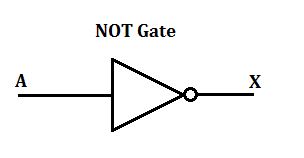
\includegraphics{../Assets/not_gate.png}

Algebra: $y=\overline x$

Tabla de verdad:
$$\begin{array}{c|c}
		x & y \\ \hline
		0 & 1 \\
		1 & 0 \\
	\end{array}$$

\section{And}

Algebra: $y=x_1 \cdot x_2$

Tabla de verdad:
$$\begin{array}{cc|c}
		x_1 & x_2 & y \\ \hline
		0   & 0   & 0 \\
		0   & 1   & 0 \\
		1   & 0   & 0 \\
		1   & 1   & 1
	\end{array}$$


\section{Or}

Algebra: $y=x_1 + x_2$

Tabla de verdad:
$$\begin{array}{cc|c}
		x_1 & x_2 & y \\ \hline
		0   & 0   & 0 \\
		0   & 1   & 1 \\
		1   & 0   & 1 \\
		1   & 1   & 1 \\
	\end{array}$$


\section{ExOr}

Algebra: $y=x_1 \oplus x_2$

Tabla de verdad:
$$\begin{array}{cc|c}
		x_1 & x_2 & y \\ \hline
		0   & 0   & 0 \\
		0   & 1   & 1 \\
		1   & 0   & 1 \\
		1   & 1   & 0 \\
	\end{array}$$

\section{NAND, NOR, XNOR}

Son iguales que el AND, OR y EXOR respectivamente, pero tienen un NOT posteriormente.

\chapter{Circuitos combinatorios}

\section{Sumador de 1 bit con compuertas logicas}

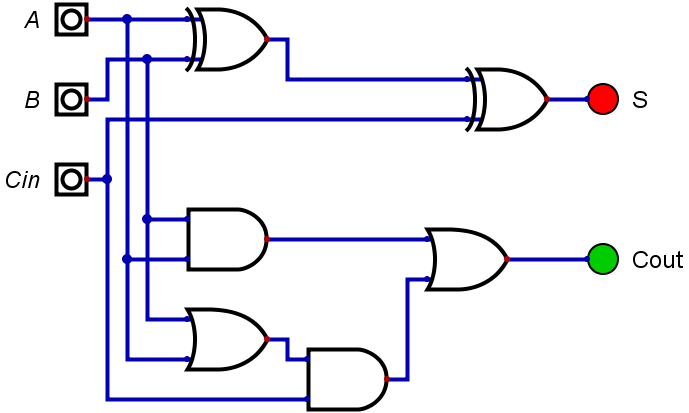
\includegraphics[width=8cm]{../Assets/SumadorCompleto.png}

El $\sum$ representa el $s_i$

\section{Mulfiplexor de 16:1}
Tenemos 16 canales, todos conectados al multiplexor y tenemos 4 entradas que determinan
cual de los canales es el que esta conectado a la salida.
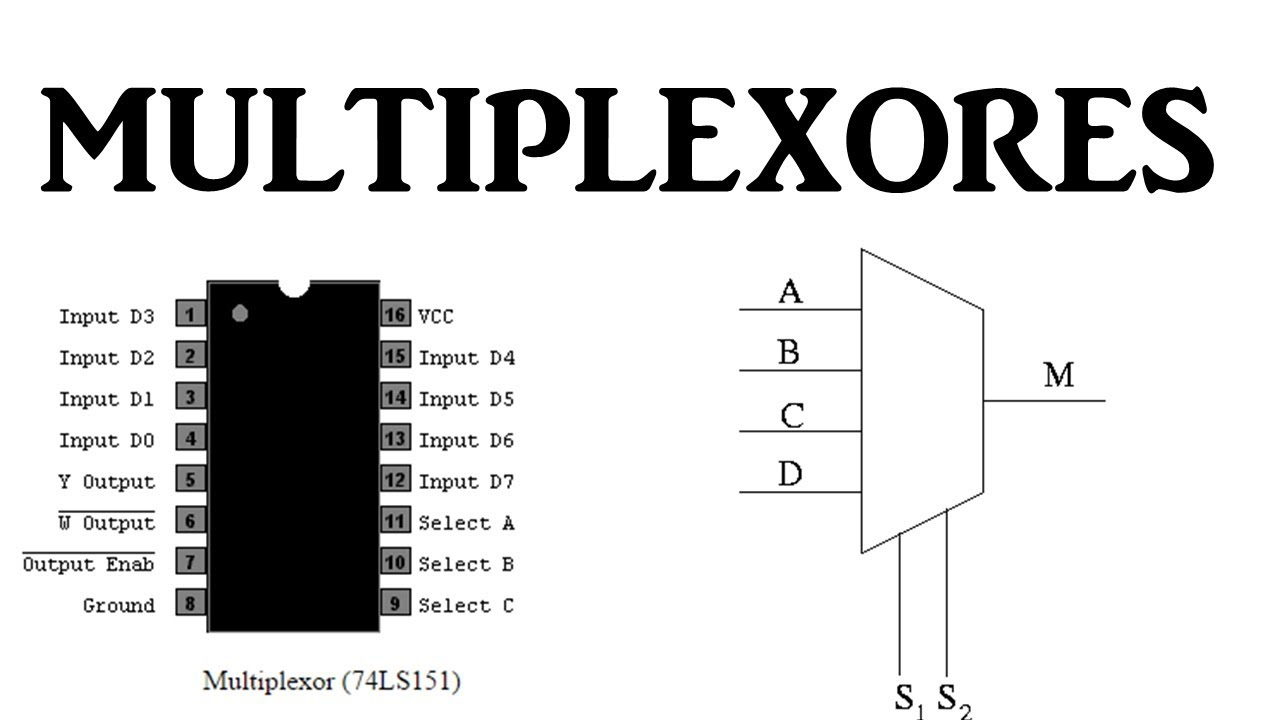
\includegraphics[width=10cm]{../Assets/multiplexor.jpg}

\section{Canalera combinatoria}

Tenemos un control de canalera, que conecta cada uno de los botones con el multiplexor y se encarga de convertir, por ejemplo, las 16 entradas del control en 4 señales que necesita el multiplexor.

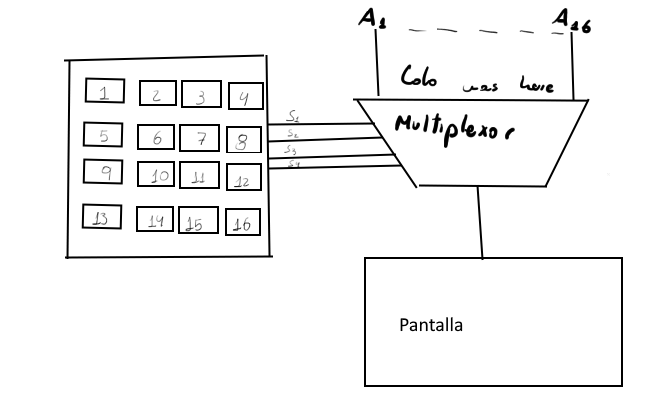
\includegraphics[width=10cm]{../Assets/canalera_combinatoria_19-03-24.png}

En este ejemplo, el canal mostrado en panatalla depende unicamente del boton presionado en el momento.

\section{Canalera secuencial}

Tenemos un control de canalera, pero en lugar de tener un boton por cada canalera, tenemos dos botones, uno para arriba y otro para abajo.
Tiene un ``Contador`` y lo que ocurre al presionar un boton es que este contador es modificado.

Los circuitos secuenciales incluyen una memoria y un estado.
El estado es toda informacion del pasado necesaria para determinar el comportamiento futuro. \
La salida depende de la entrada en el momento dado y del estado del circuito.



\section{Funciones logicas}

Es un circuito que dado un conjunto de entradas X genera un conjunto de entradas Y que depende de dichas entradas. Es por esto que se le llama funcion logica.\
Representamos las Funciones Logicas (FL) con tablas de verdad o con las expresiones algebraicas. Tambien tenemos el formato esquematico que es a lo que desea llegar para poder construir los circuitos.
Pasar de los Requerimientos (del cliente o del entregable) al Esquematico es llamado Síntesis. Pasar del Esquematico a los Requerimientos es llamado Análisis.
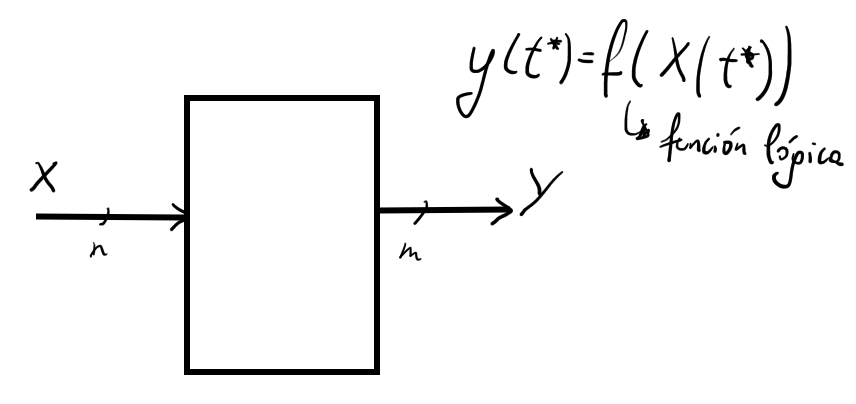
\includegraphics[width=10cm]{../Assets/circuitos_combinatorios2.png}

\section{Representacion Canonica de FL}


Sean $\{x_{n-1},...,x_0\}$ entradas de una FL.\
Sea $y_i$ la salida de una de las $m$ FL.

Un $\underline{literal}$ es una entrada ($x_i$) o su negado ($\overline{x_i}$).\
Un \underline{término producto} es el producto de uno o mas literales.\
Un \underline{minitérmino} es un término producto que involucra todas las entradas.

$$m_0 = \overline{x_2} \cdot \overline{x_1} \cdot \overline{x_0}$$
$$m_1 = \overline{x_2} \cdot \overline{x_1} \cdot x_0$$
$$m_2 = \overline{x_2} \cdot x_1  \cdot \overline{x_0}$$
$$m_3 = \overline{x_2} \cdot x_1  \cdot x_0$$
$$m_4 = x_2  \cdot \overline{x_1} \cdot \overline{x_0}$$
$$m_5 = x_2  \cdot \overline{x_1} \cdot x_0$$
$$m_6 = x_2  \cdot x_1  \cdot \overline{x_0}$$
$$m_7 = x_2  \cdot x_1  \cdot x_0$$

$$\begin{array}{ccc|cccccccc|c}
		x_2 & x_1 & x_0 & m_0 & m_1 & m_2 & m_3 & m_4 & m_5 & m_6 & m_7 & y_i \\ \hline
		0   & 0   & 0   & 1   & 0   & 0   & 0   & 0   & 0   & 0   & 0   & 0   \\
		0   & 0   & 1   & 0   & 1   & 0   & 0   & 0   & 0   & 0   & 0   & 0   \\
		0   & 1   & 0   & 0   & 0   & 1   & 0   & 0   & 0   & 0   & 0   & 1   \\
		0   & 1   & 1   & 0   & 0   & 0   & 1   & 0   & 0   & 0   & 0   & 0   \\
		1   & 0   & 0   & 0   & 0   & 0   & 0   & 1   & 0   & 0   & 0   & 0   \\
		1   & 0   & 1   & 0   & 0   & 0   & 0   & 0   & 1   & 0   & 0   & 1   \\
		1   & 1   & 0   & 0   & 0   & 0   & 0   & 0   & 0   & 1   & 0   & 1   \\
		1   & 1   & 1   & 0   & 0   & 0   & 0   & 0   & 0   & 0   & 1   & 1   \\
	\end{array}$$

En este caso, $y_i$ es una FL cualquiera, para poder calcularla, debemos sumar miniterminos.

$$y_i = m_2 + m_5 + m_6 + m_7 $$
$$y_i = \overline{x_2} \cdot x_1 \cdot \overline{x_0} + x_2 \cdot \overline{x_1} \cdot x_0 + x_2 \cdot x_1 \cdot \overline{x_0} + x_2 \cdot x_1 \cdot x_0$$

Recordando la tabla del sumador de 1 bit:


$$\begin{array}{ccc|cc}
		a_i & b_i & C_{in_i} & C_{out_i} & s_i \\ \hline
		0   & 0   & 0        & 0         & 0   \\
		0   & 0   & 1        & 0         & 1   \\
		0   & 1   & 0        & 0         & 1   \\
		0   & 1   & 1        & 1         & 0   \\
		1   & 0   & 0        & 0         & 1   \\
		1   & 0   & 1        & 1         & 0   \\
		1   & 1   & 0        & 1         & 0   \\
		1   & 1   & 1        & 1         & 1   \\
	\end{array}$$


Podemos escribir:
$$ C_{out_i} = m_3 + m_5 + m_6 + m_7 =
	\overline{x_2} \cdot x_1  \cdot x_0 +
	x_2  \cdot \overline{x_1} \cdot x_0 +
	x_2  \cdot x_1  \cdot \overline{x_0} +
	x_2  \cdot x_1  \cdot x_0
$$
$$ s_i = m_1 + m_2 + m_4 + m_7 =
	\overline{x_2} \cdot \overline{x_1} \cdot x_0 +
	\overline{x_2} \cdot x_1  \cdot \overline{x_0} +
	x_2  \cdot \overline{x_1} \cdot \overline{x_0} +
	x_2  \cdot x_1  \cdot x_0
$$
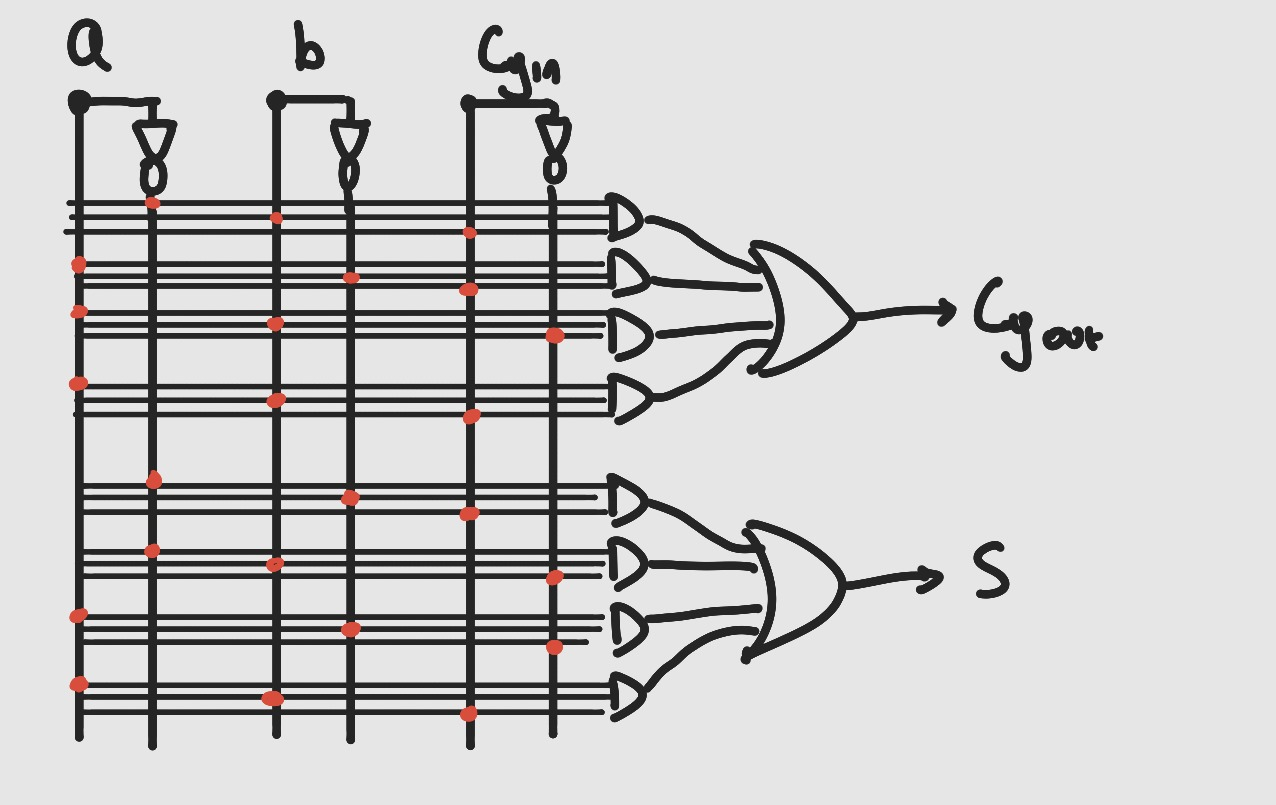
\includegraphics[width=10cm]{../Assets/sumador_de_1bit.jpeg}
% creditos alfonso

\section{Definicion}

Un \underline{término suma} es la suma de uno o mas literales.\
Un \underline{maxitérmino} es un término suma que involucra todas las entradas.

$$M_0 = x_2  + x_1  + x_0$$
$$M_1 = x_2  + x_1  + \overline{x_0}$$
$$M_2 = x_2  + \overline{x_1} + x_0$$
$$M_3 = x_2  + \overline{x_1} + \overline{x_0}$$
$$M_4 = \overline{x_2} + x_1  + x_0$$
$$M_5 = \overline{x_2} + x_1  + \overline{x_0}$$
$$M_6 = \overline{x_2} + \overline{x_1} + x_0$$
$$M_7 = \overline{x_2} + \overline{x_1} + \overline{x_0}$$

$$\begin{array}{ccc|cccccccc|c}
		x_2 & x_1 & x_0 & M_0 & M_1 & M_2 & M_3 & M_4 & M_5 & M_6 & M_7 & y_i \\ \hline
		0   & 0   & 0   & 0   & 1   & 1   & 1   & 1   & 1   & 1   & 1   & 0   \\
		0   & 0   & 1   & 1   & 0   & 1   & 1   & 1   & 1   & 1   & 1   & 0   \\
		0   & 1   & 0   & 1   & 1   & 0   & 1   & 1   & 1   & 1   & 1   & 1   \\
		0   & 1   & 1   & 1   & 1   & 1   & 0   & 1   & 1   & 1   & 1   & 0   \\
		1   & 0   & 0   & 1   & 1   & 1   & 1   & 0   & 1   & 1   & 1   & 0   \\
		1   & 0   & 1   & 1   & 1   & 1   & 1   & 1   & 0   & 1   & 1   & 1   \\
		1   & 1   & 0   & 1   & 1   & 1   & 1   & 1   & 1   & 0   & 1   & 1   \\
		1   & 1   & 1   & 1   & 1   & 1   & 1   & 1   & 1   & 1   & 0   & 1   \\
	\end{array}$$

En este caso:
$$ y_i = M_0 \cdot M_1 \cdot M_3 \cdot M_4 $$

Para hacer con los maxiterminos tenes que poner los que te quedan con 0, mientras que para hacer con los miniterminos tenes que poner los que te quedan con 1.\
``
Si te dan una FL para hacer el algebra, escribir las dos y usar la que tenga menos terminos.
``


\section{Algebra de Boole}

\section{Axioma 1}

Sea $x$ una variable booleana $\Rightarrow \begin{cases}
		x=0 \Rightarrow x\ne 1 \\
		x=1 \Rightarrow x\ne 0 \\
	\end{cases}$

\section{Axioma 2}

Sea $x$ e $y$ variables booleanas \\ $y=\bar{x}\Rightarrow
	\begin{array}{c|c}
		x & y \\ \hline
		0 & 1 \\
		1 & 0 \\
	\end{array}$

\section{Axioma 3}

Sean $x_1 , x_0$ e $y$ variables booleanas \\
$$\begin{cases}
		y = x_1 + x_0 \Rightarrow
		\begin{array}{cc|c}
			x_1 & x_0 & y \\ \hline
			0   & 0   & 0 \\
			0   & 1   & 1 \\
			1   & 0   & 1 \\
			1   & 1   & 1 \\
		\end{array} \\
		y = x_1 \cdot x_0 \Rightarrow
		\begin{array}{cc|c}
			x_1 & x_0 & y \\ \hline
			0   & 0   & 0 \\
			0   & 1   & 0 \\
			1   & 0   & 0 \\
			1   & 1   & 1 \\
		\end{array}
	\end{cases}
$$


\section{Propiedades del algebra de Boole}


1. Asociativa OR: $x_2 + (x_1 + x_0) = (x_2 + x_1) +x_0$
2. Conmutativa OR: $x_2 + x_1 = x_1 + x_2$
3. Asociativa AND: $x_2 \cdot (x_1 \cdot x_0) = (x_2 \cdot x_1) \cdot x_0$
4. Conmutativa AND: $x_2 \cdot x_1 = x_1 \cdot x_2$


\section{LEY K}

Sean $a,b$ variables booleanas, se cumple que $a\cdot b + a\cdot \bar{b} = a$

\section{Demostracion por induccion perfecta}

$$
	\begin{array}{cc|c|c|c}
		a & b & a \cdot b & a \cdot \bar{b} & a \cdot b + a \cdot \bar{b} \\ \hline
		0 & 0 & 0         & 0               & 0                           \\
		0 & 1 & 0         & 0               & 0                           \\
		1 & 0 & 0         & 1               & 1                           \\
		1 & 1 & 1         & 0               & 1                           \\
	\end{array}
$$

\section{Leyes de Morgan}

$$\overline{x_1 \cdot x_0} = \overline{x_1} + \overline{x_0}$$
$$\overline{(x_1 + x_0)} = \overline{x_1} \cdot \overline{x_0}$$

\section{Mapas de Karnaugh}

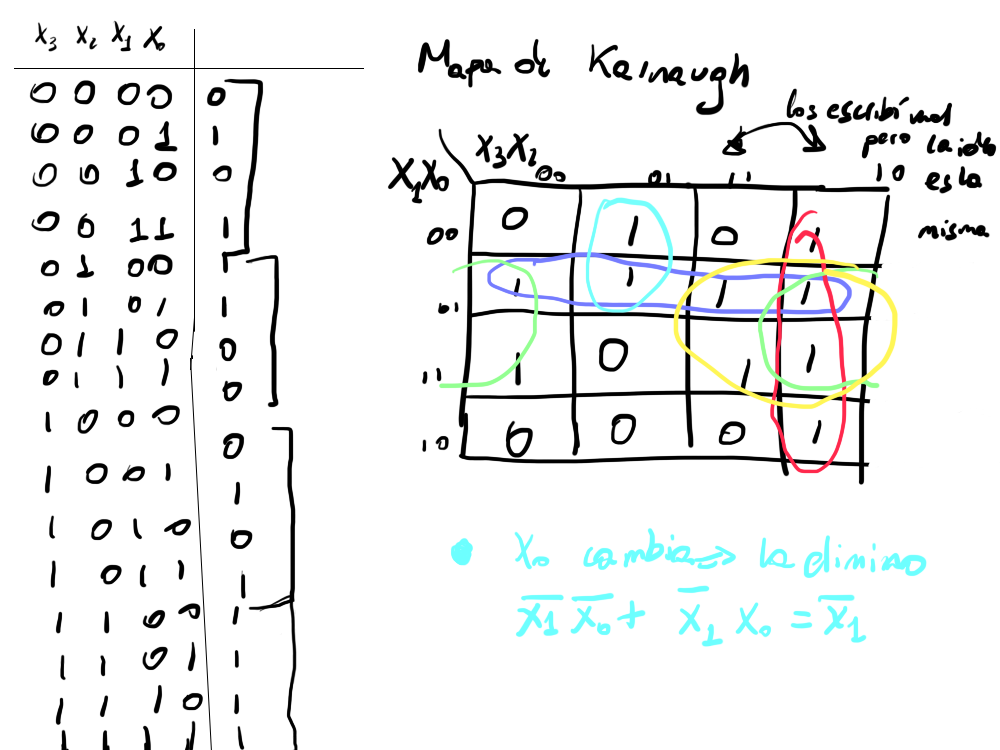
\includegraphics[width=10cm]{../Assets/mapas_de_karnaugh.png}

\section{Minizmizacion de funciones logicas}

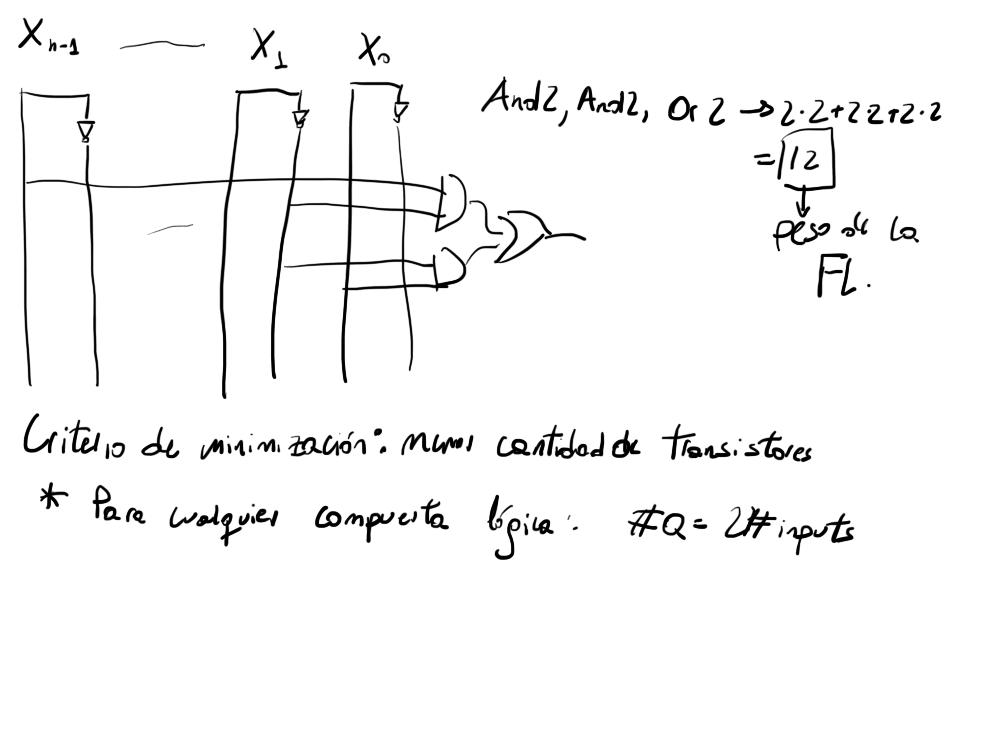
\includegraphics[width=10cm]{../Assets/peso_fl.png}

Buscamos minimizar la cantidad de entradas del primer nivel y del segundo nivel.
Pero minimizar la cantidad de entradas del segundo nivel es minimizar la cantidad de salidas del segundo nivel.
Para esto vamos a minimizar la cantidad de literales del primer nivel y minimizar la cantida de compuertas del primer nivel.

\section{Pasos de minimizacion}

\begin{enumerate}
	\item Hallar los implicantes primos. En los mapas de karnaugh es hallar los grupos de 1s mas grandes
	\item Hallar las celdas 1 distinguidas. Esto es hallar las celdas que tienen 1s que solo aparecen en un grupo.
	\item Suma de implicantes primos esenciales. Esto es las expresiones minimas que aportan a las celdas distinguidas.
\end{enumerate}

\chapter{Circuitos Secuenciales}
\section{Definicion}
Los circuitos secuenciales son circuitos cuya salida no solo dependen de la entrada en un determinado instante sino que tambien dependen de un estado.

Para lograr esto, veremos distintos elementos de memoria que nos ayudan a almacenar el estado.

\section{Arquitectura general de un circuito secuencial}

Un circuito secuencial tiene tres componentes principales: la logica del estado actual, los elementos de memoria y la logica de salida. Los estados de memoria tienen como entrada el estado actual. El estado actual depende tanto del elemento de memoria (que sera el estado siguiente) como de las entradas de todo el circuito. Por ultimo, la logica de salida depende de la entrada y los elementos de memoria.


\chapter{Elementos de memoria}

\section{Biestable}
El primer elemento que de memoria que veremos es el biestable.

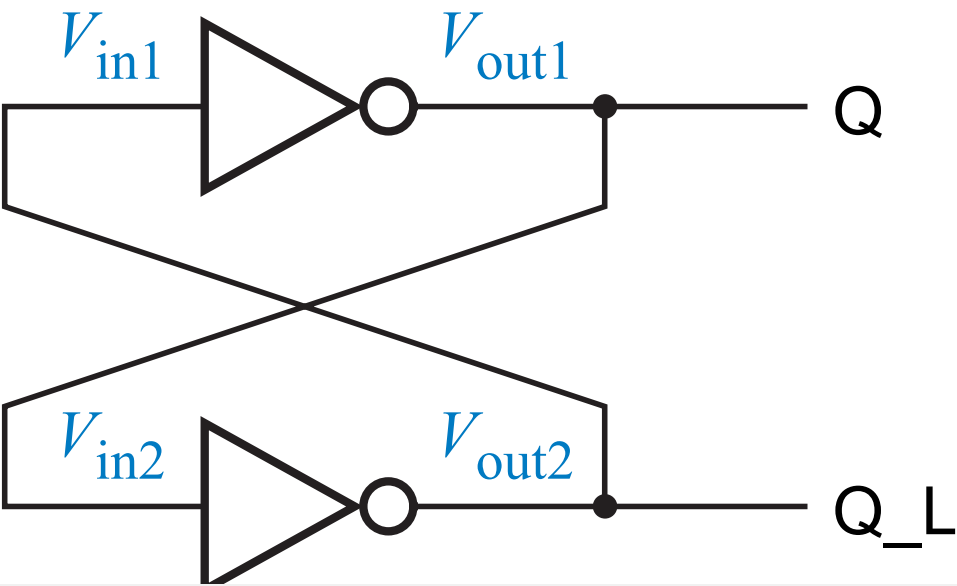
\includegraphics[width=6cm]{../Assets/bistable.png}

\section{Latch-SR}

 (Este es distinto al Latch-SR que dimos en clase) \

Podemos modificar el Biestable para tener dos entradas, S y R, que nos permiten Settear y Resettear el estado Q.

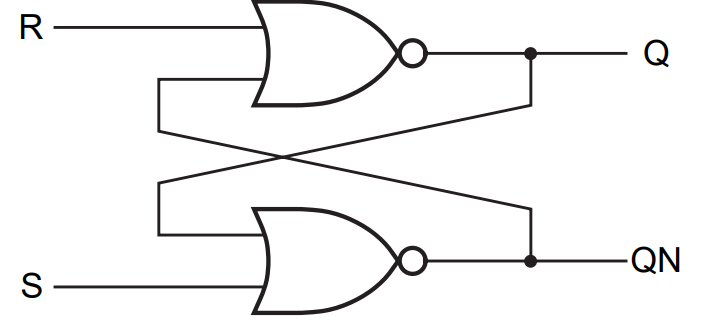
\includegraphics[width=6cm]{../Assets/latch-sr.png}

Aca tampoco ocurre que $Q=\overline{QN} \leftarrow$ \
$\begin{array}{cc|cc}
		S & R & Q     & QN     \\ \hline
		0 & 0 & lastQ & lastQN \\
		0 & 1 & 0     & 1      \\
		1 & 0 & 1     & 0      \\
		1 & 1 & 0     & 0      \\
	\end{array}$


\section{Latch-$S_L-R_L$}

 (Este no lo dimos en clase) \\
(A partir del Latch-SR la implementacion de compuertas es distinta a como la dimos en clase pero el funcionamiento es el mismo)\\
El Latch-$\overline{SR}$ es igual que el Latch SR solo que con entradas negadas. En esencia funciona de manera contraria a como funciona el Latch-SR pero la idea es la misma

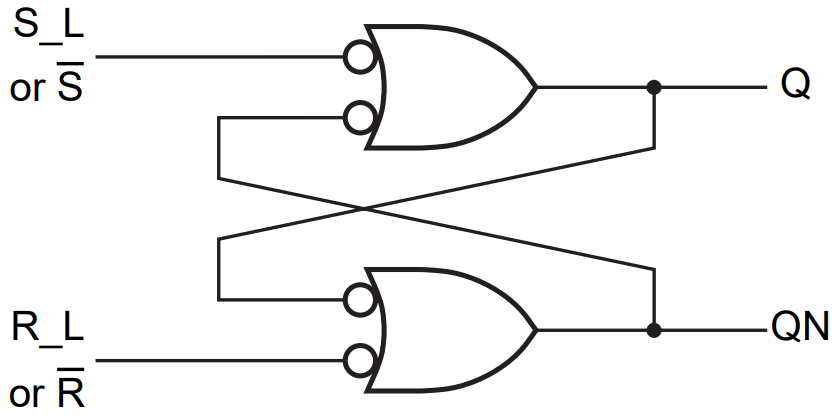
\includegraphics[width=6cm]{../Assets/latch-sl-rl.png}

\section{Latch-SR con enable}
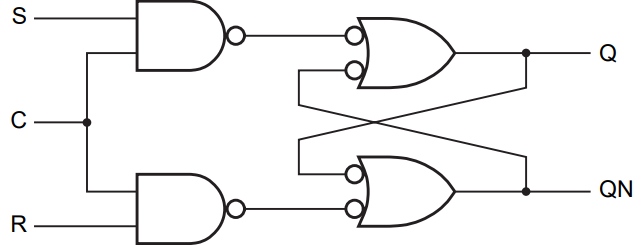
\includegraphics[width=6cm]{../Assets/latch-sr-con-enable.png}

En esencia todo lo que hace el enable (C) es que no se permita el uso del S o R en todo momento sino que solo cuando esta habilitado.


\section{Latch-D}
El latch-D sustituye el S y R y representa una cierta Data que queremos almacenar.

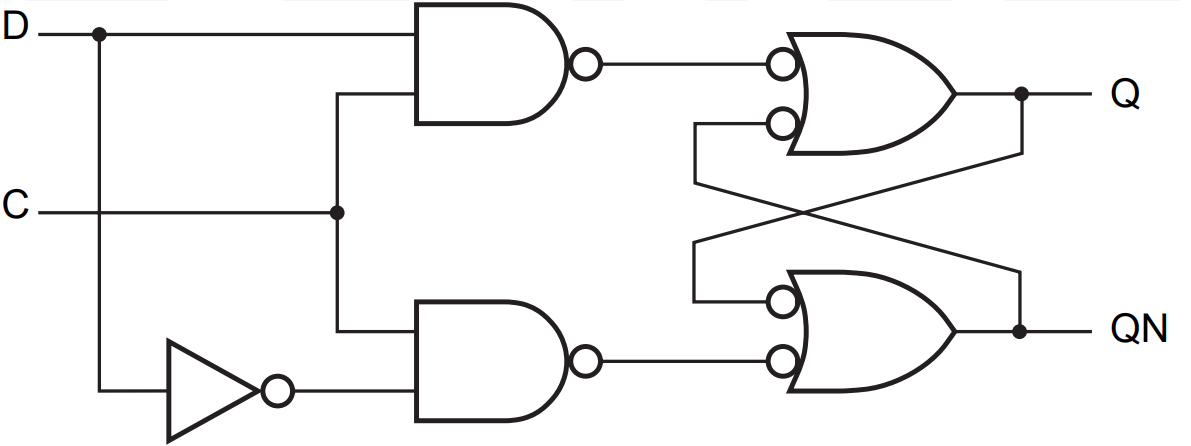
\includegraphics[width=6cm]{../Assets/latch-d.png}

$$\begin{array}{cc|cc}
		C & D & Q     & QN     \\ \hline
		1 & 0 & 0     & 1      \\
		1 & 1 & 1     & 0      \\
		0 & x & lastQ & lastQN \\
	\end{array}$$ \\

Este circuito se representa asi: \\
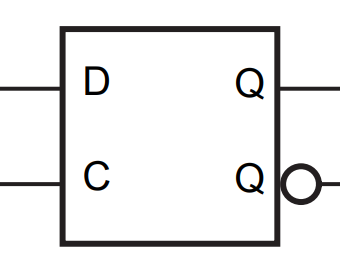
\includegraphics[width=2cm]{../Assets/latch-d-rep.png}

\section{D-FlipFlop}

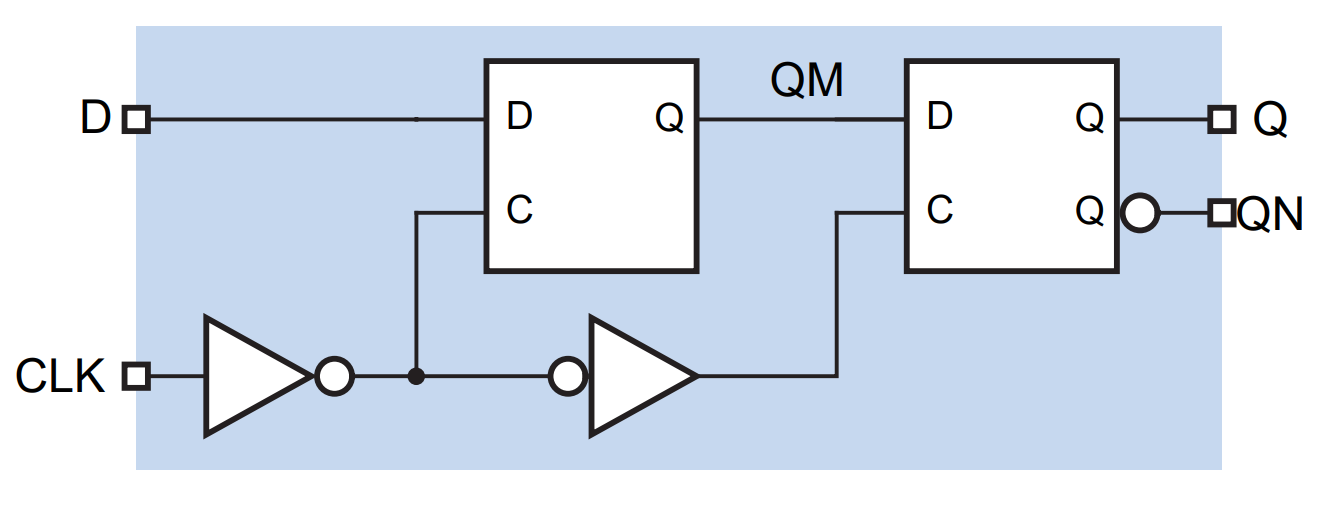
\includegraphics[width=6cm]{../Assets/d-flipflop.png}

$\begin{array}{cc|cc}
		D & CLK                                                                & Q     & QN     \\ \hline
		0 & \texttiming{[timing/c/rising arrows,timing/c/arrow pos =.7]{2{C}}} & 0     & 1      \\ % the second term is just to draw the rising edge 
		1 & \texttiming{[timing/c/rising arrows,timing/c/arrow pos =.7]{2{C}}} & 1     & 0      \\
		x & 0                                                                  & lastQ & lastQN \\
		x & 1                                                                  & lastQ & lastQN \\
	\end{array}$

\chapter{Microprocesadores}
\section{Arquitectura general de los microprocesadores}
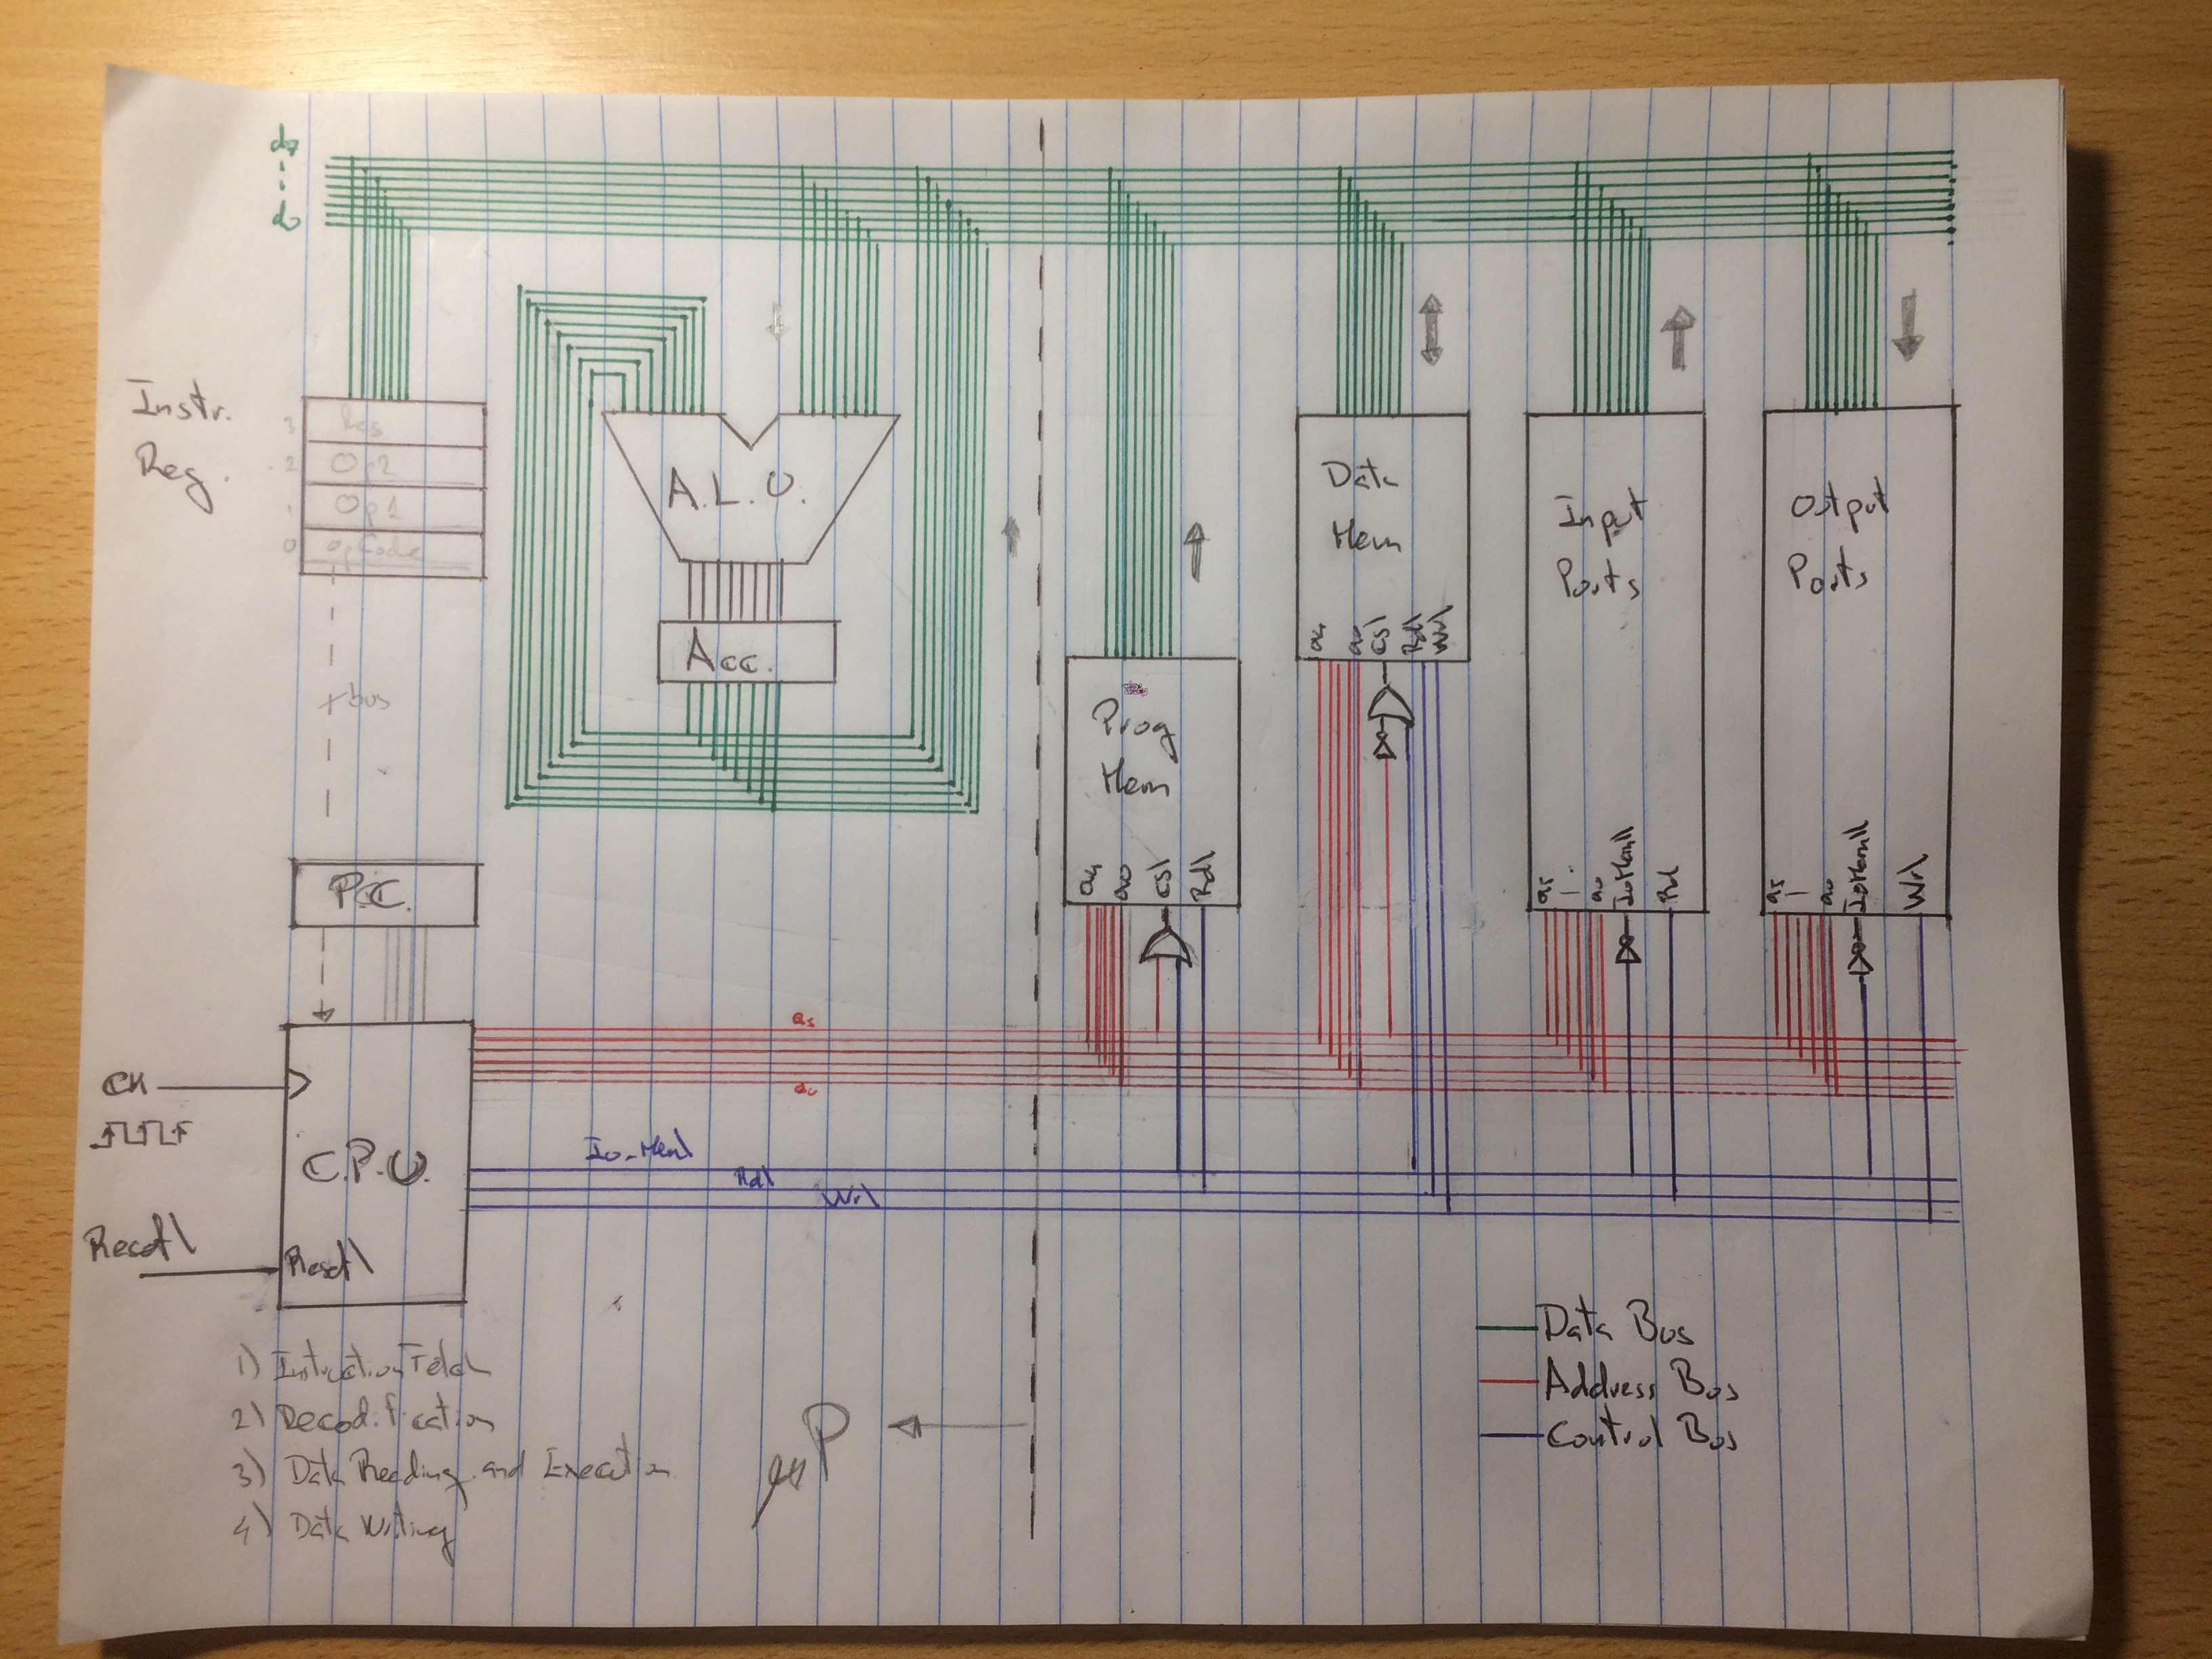
\includegraphics[width=8cm]{../Assets/arquitectura_general_uP.JPG}

El Address Bus y el Control Bus tienen un tamaño que puede variar. \\
En la realidad, Program memory y el Data memory van en una sola memoria. Se está separando para marcar que conceptualmente son dos cosas distintas.\\
La altura de la memoria es la Capacidad de direccionamiento. El ancho de la memoria es el Ancho de palabra.\\
\newpage
Visto de manera simplificada, tenemos el siguiente esquema:\\

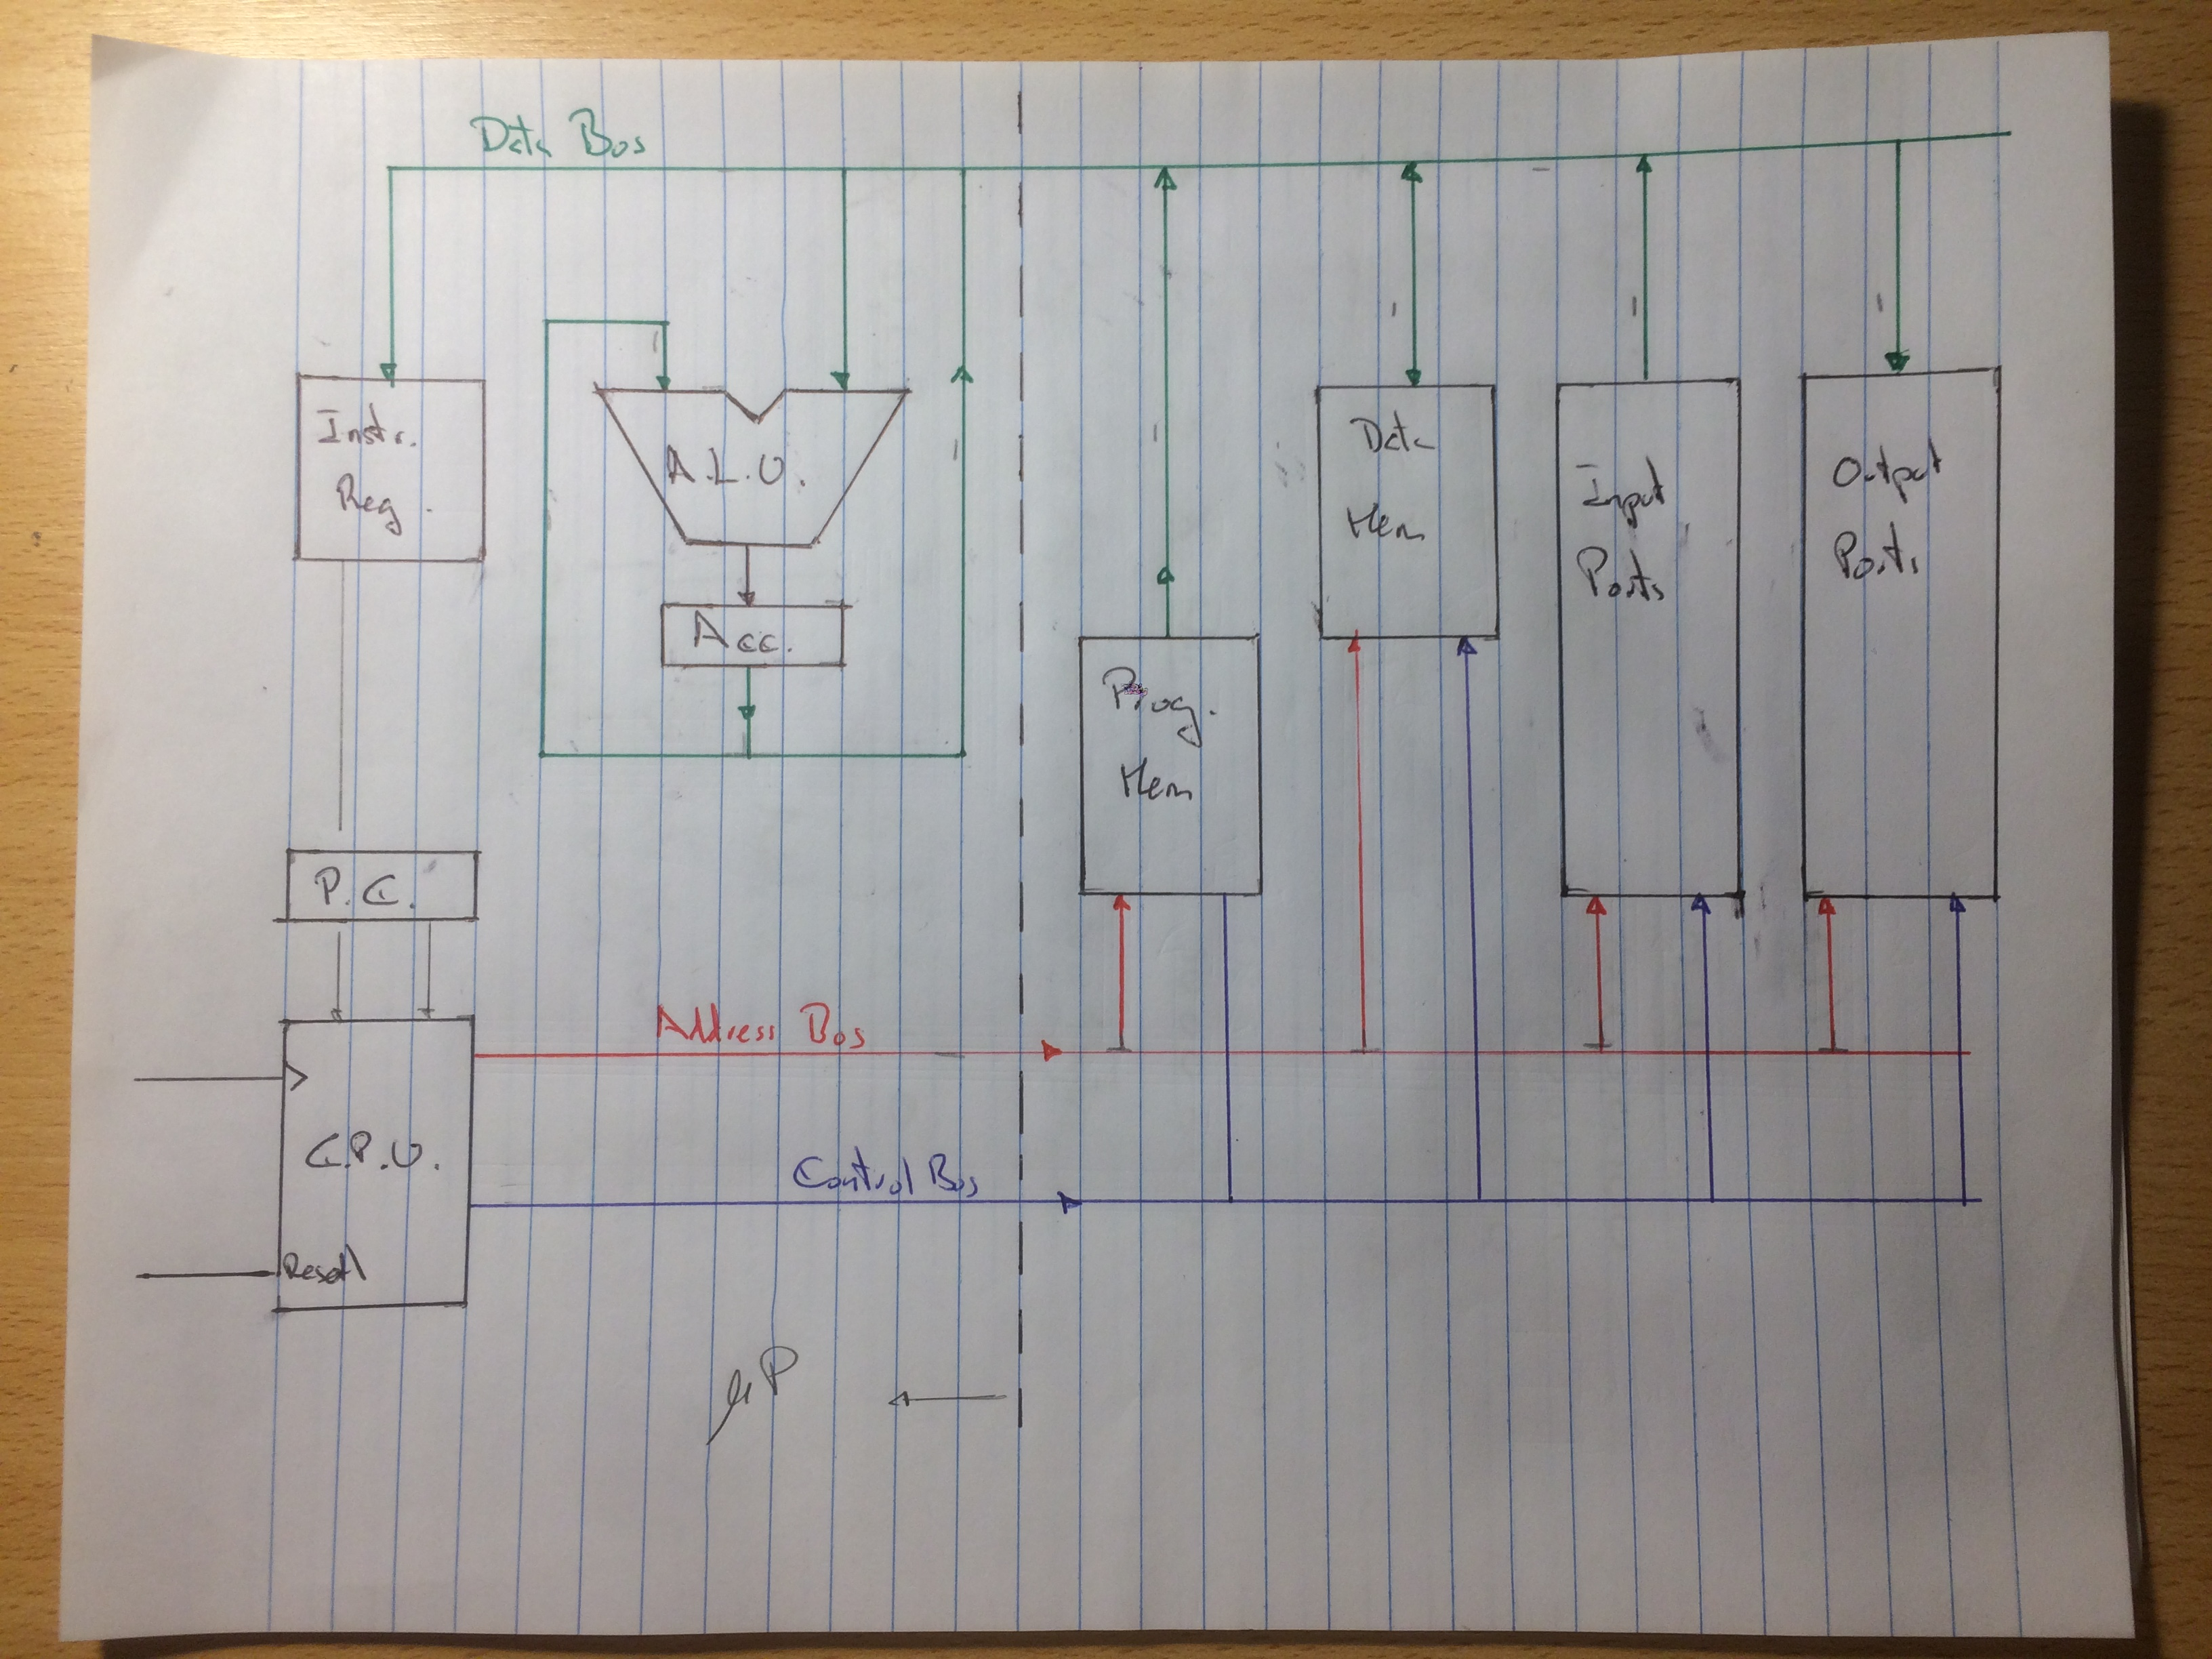
\includegraphics[width=8cm]{../Assets/arquitectura_simplificada_uP.jpg}

\section{Funcionamiento}

El \(\mathbb{PC}\) es el Program Counter. Indica qué intstrucción es la que se está ejecutando.

Luego de un Reset\(\setminus\)
\begin{enumerate}
	\setcounter{enumi}{-1}
	\item \(\mathbb{PC}\) = 0x00.
	\item Instruction Fetch.
	\item Decode.
	\item Lectura de datos y Extracción \(\rightarrow\) Memory In Ports.
	\item Escritura de datos \(\rightarrow\) Memory Out Ports.
	\item \(\mathbb{PC}\)++ y volver a instrucción 1.
\end{enumerate}

\section{Set de instrucciones}
Vamos a crear nuestro propio \(\mu P\)

Asignamos 6 bits a la capacidad de direccionamiento y 8 bits al ancho de palabra.
Esto significa que tenemos 64 registros en nuestra memoria y las palabras miden 1 byte.
\newpage
El posible set de instrucciones es:\\
\[
	\begin{array}{|llll|l|} \hline
		Operacion & Entrada1               & Entrada2 & Salida  & NumInstruccion \\ \hline
		Add       & Op1                    & Op2      & Res     & 00000000       \\ \hline
		Sub       & Op1                    & Op2      & Res     & 00000001       \\ \hline
		And       & Op1                    & Op2      & Res     & 00000010       \\ \hline
		Or        & Op1                    & Op2      & Res     & 00000011       \\ \hline
		If        & X                      & Op       & bit     & 00000100       \\
		          & \begin{array}{ll}
			            True  & Instruction \\
			            False & Instruction \\
		            \end{array} &          &         &                           \\ \hline
		Goto      & X                      & X        & Address & 00000101       \\ \hline
	\end{array}
\] \\
El \(Op1\), \(Op2\), etc se ven así: \\
\[
	\underbrace{b_7}_{\mathclap{
		\begin{array}{c}
			0: \text{Memory} \\
			1: \text{In/Out}
		\end{array}
	}
	}
	\overbrace{b_6}^{\mathclap{
		\begin{array}{c}
			0: \text{Memory o In/Out} \\
			1: \text{Constante (Cte)}
		\end{array}
	}
	}
	\underbrace{b_5b_4b_3b_2b_1b_0}_{\mathclap{\text{Reg}}}
\]

Si el segundo bit (\(b_6\)) es 1, se determina si es In o Out por contexto. Si se esta colocaldo como un byte de entrada sera del In. Si esta en un byte de salida sera del Out.

Sin embargo, si tenemos las siguientes instrucciones:\\

\[
	\begin{array}{llll}
		Sub, & Inx24, & Cted17, & Memd64 \\
		If,  & X,     & Memd64, & bit    \\
	\end{array} \\
\]

Esto se traduce en binario a:\\

\[
	\begin{array}{llll}
		00000001, & 01100100,          & 1\texttt{X}010001, & 00111111 \\
		00000100, & \texttt{XXXXXXXX}, & 00111111,          & 00000111 \\
	\end{array}
\]

Veamos como quedan las instrucciones en memoria:\\

\[
	\begin{array}{|c|l}
		\vdots            &                           \\
		00000100          & \rightarrow \mathbb{PC}+1 \\ \hline
		00111111          &                           \\ \hline
		1\texttt{X}010001 &                           \\ \hline
		01100100          &                           \\ \hline
		00000001          & \rightarrow \mathbb{PC}   \\ \hline
	\end{array}
\]

\section{Clasificacion de microprocesadores}

Hay dos clasificaciones:\\
\begin{enumerate}
	\item Organizacion de memoria
	\item Instruction set
\end{enumerate}
\subsection{Segun la Organizacion de memoria}
Recordemos primero que las operaciones que realiza el microprocesador:
\begin{enumerate}
	\item Instruction Fetch
	\item Decode
	\item Data reading
	\item Data reading and execute
	\item Data writing
\end{enumerate}
{\large Arquitectura Von Neumann} \\
El microprocesador tiene una sola memoria que engloba tanto el Data Memory como el Program Memory. \\
Las operaciones se realizaran de esta manera:
\[
	\begin{array}{l|l|l|l|l}
		Instruction1 & 1,2 & 3,4 &     &     \\
		Instruction2 &     &     & 1,2 & 3,4 \\
	\end{array}
\]
Tenemos que hacer cada instruccion de manera secuencial. \\

{\large Arquitectura de Harvard} \\
La memoria del microprocesador tiene dos memorias separadas fisicamente, una para el Data Memory y otra para el Program Memory. \\
Las operaciones se realizaran de esta manera:
\[
	\begin{array}{l|l|l|l|l}
		Instruction1 & 1,2 & 3,4 &     & \\
		Instruction2 &     & 1,2 & 3,4 & \\
	\end{array}
\]
\newpage

\begin{table}[ht]
	\centering
	\begin{tabular}{p{0.5\linewidth}|p{0.5\linewidth}}
		Von Neuman                                        & Harvard                                           \\ \hline
		No permite pipeline                               & Permite pipeline                                  \\ \hline
		1 solo Address Bus y 1 solo Data Bus              & 2 Adress Bus y 2 Data Bus                         \\ \hline
		Existe problema de estructura en Program Memory   & No existe problema de escritura en Program Memory \\ \hline
		Flexibilidad en cantidad de Program y Data Memory & No flexible                                       \\
	\end{tabular}
	\caption{Tabla comparativa}
	\label{tab:clas_uP_org_mem}
\end{table}

\subsection{Segun el Instruction Set}
{\large RISC}: Reduced Instruction Set Computer \\

{\large CISC}: Complex Instruction Set Computer


\end{document}
